\documentclass[a4paper, 12pt]{report}

\usepackage{cmap}
\usepackage[T1, T2A]{fontenc}
\usepackage[utf8]{inputenc}
\usepackage[english, russian]{babel}

\usepackage{graphicx, graphics}
\usepackage{float}
\usepackage{wrapfig}
\graphicspath{{image/}}

\usepackage[left=20mm, top=15mm, right=20mm, bottom=10mm, nohead, footskip=7mm]{geometry}

\usepackage{color} %May be necessary if you want to color links 
\usepackage{hyperref} 
\hypersetup{ colorlinks=true, %set true if you want colored links 
linktoc=all, %set to all if you want both sections and subsections linked 
linkcolor=blue, %choose some color if you want links to stand out 
}

\author{Кривонос Анна \\ 317 группа}
\title{Практическое задание \\ Композиции алгоритмов для решения задачи регрессии }


\begin{document}

\maketitle

\tableofcontents{}
\clearpage

\chapter{Введение}
В данном отчете исследуютcя алгоритмы случайного леса и градиентного бустинга для задачи регрессии с функцией потерь RMSE.
Для тестирования моделей изпользуется дадасет данных о продажах недвижимости House Sales in King County, USA.



\chapter{Эксперименты}
Перед началом работы проведем предобработку данных. Удалим столбец 'id', так как он мало коррелирует с целевой переменнной. Также преобразуем столбец 'date' в Datetime и добавим на основе этого столбца три новых признака - день, месяц, год. После столбец 'date'
удалим. Затем разделим данные на обучающую и валидационную выборки.


\section{Исследование поведения алгоритма случайный лес.}  


Исследуем зависимость значения функции потерь на отложенной выборке и  времени работы алгоритма в зависимости от следующих параметров:
\begin{itemize}
        \item количество деревьев в ансамбле 
        \item размерность подвыборки признаков для одного дерева
        \item максимальная глубина дерева
\end{itemize}


Рассмотрим следующие параметры :
\begin{table}[H]
\begin{tabular}{lllll}
размерность подвыборки признаков: & 0.1 & 0.5 & 1 & 0.3  \\
глубина дерева:  & 1 & 5 & 10 & None  \\
\end{tabular}
\end{table}

Количество деревьев рассмотри от 1 до 100



При увеличении числа деревьев значение RMSE начинает колебаться около одного числа(рис. 2.1). Наименьшее значение точности достигается, когда размерность подвыборки равна количеству признаков в датасете. Алгоритм на каждом шаге знает все признаки, поэтому лучше настраивается на данные. При глубине 1 и features\_size=1 алгоритмы получаются похожими, поэтому точность почти не зависит от количества деревьев. Также из графика видно, что с ростом глубины значение RMSE растет, так как модель сильно подстраивается под данные и переобучается. При неограниченной глубине точность на подвыборке признаков в 10\% оказывается лучше, чем на всей выборке признаков.


\begin{figure}[H]
        	\centering
        	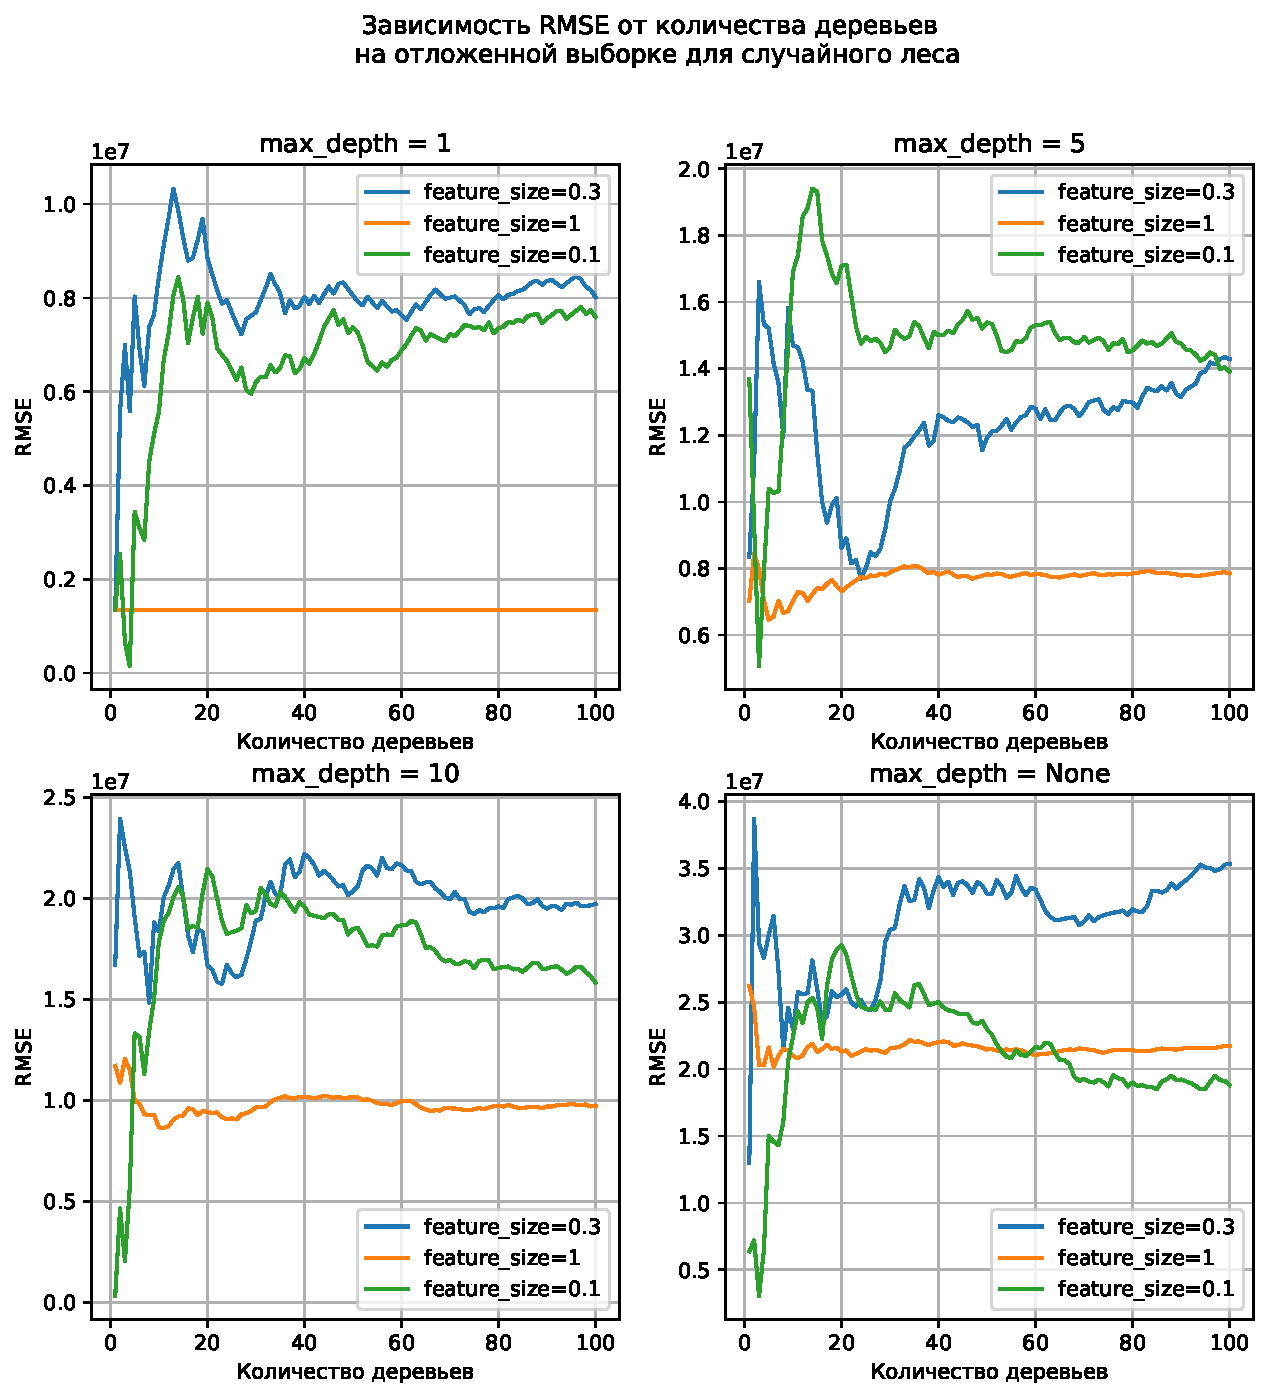
\includegraphics[width=0.7\linewidth]{ex1_1.pdf}
        	\label{fig:mpr}
        	\vspace{-25pt}
        	\caption{}


\end{figure}


С ростом числа деревьев и максимальной глубины время работы алгоритма растет. Причем при неограниченной глубине время работы почти в два раза дольше.

\begin{figure}[H]
        	\centering
        	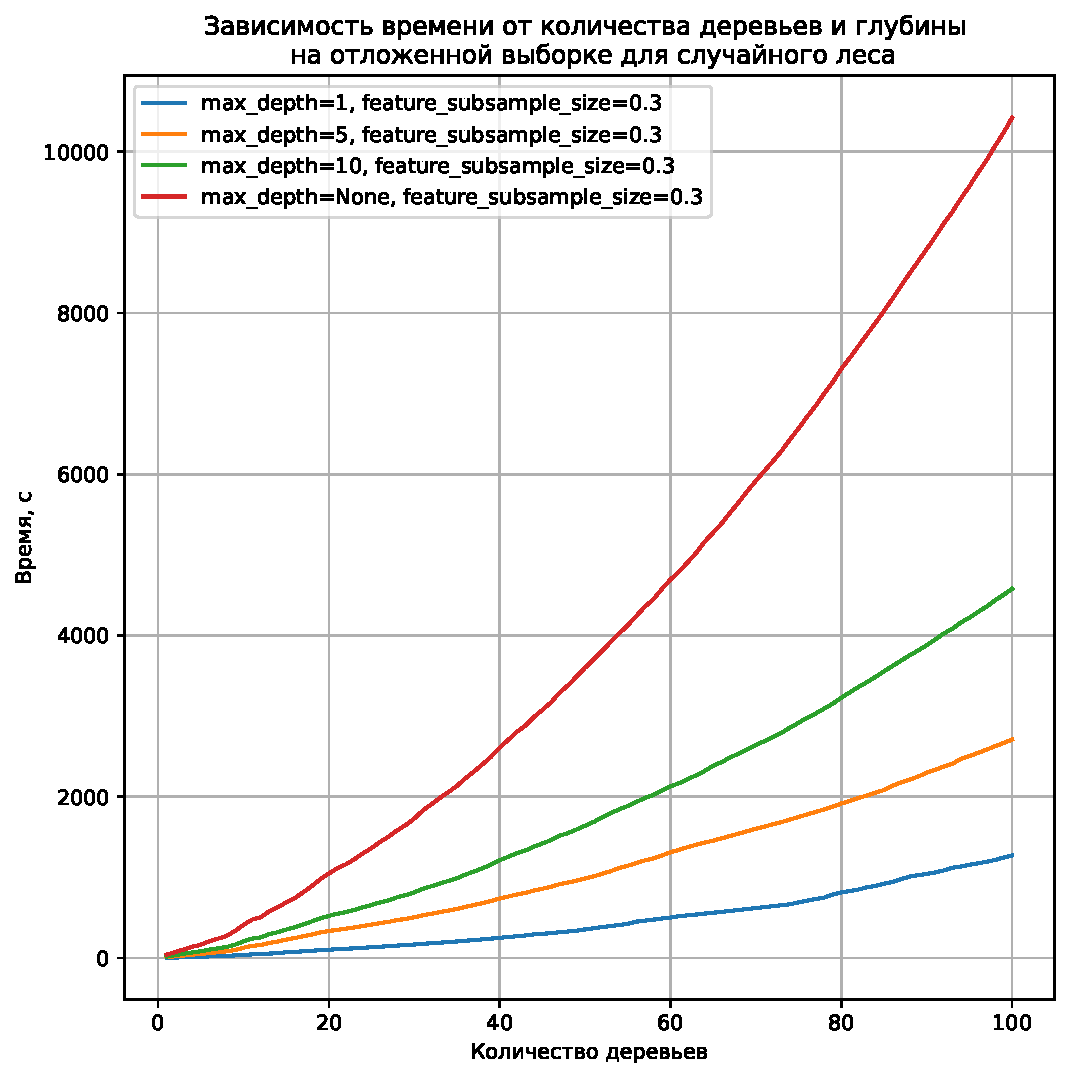
\includegraphics[width=0.73\linewidth]{ex1_2.pdf}
        	\label{fig:mpr}
        	\vspace{-23pt}
\end{figure}

Как видно из рисунка ниже, значение RMSE с ростом глубины растет, оптимальной является глубина меньше 5.

\begin{figure}[H]
        	\centering
        	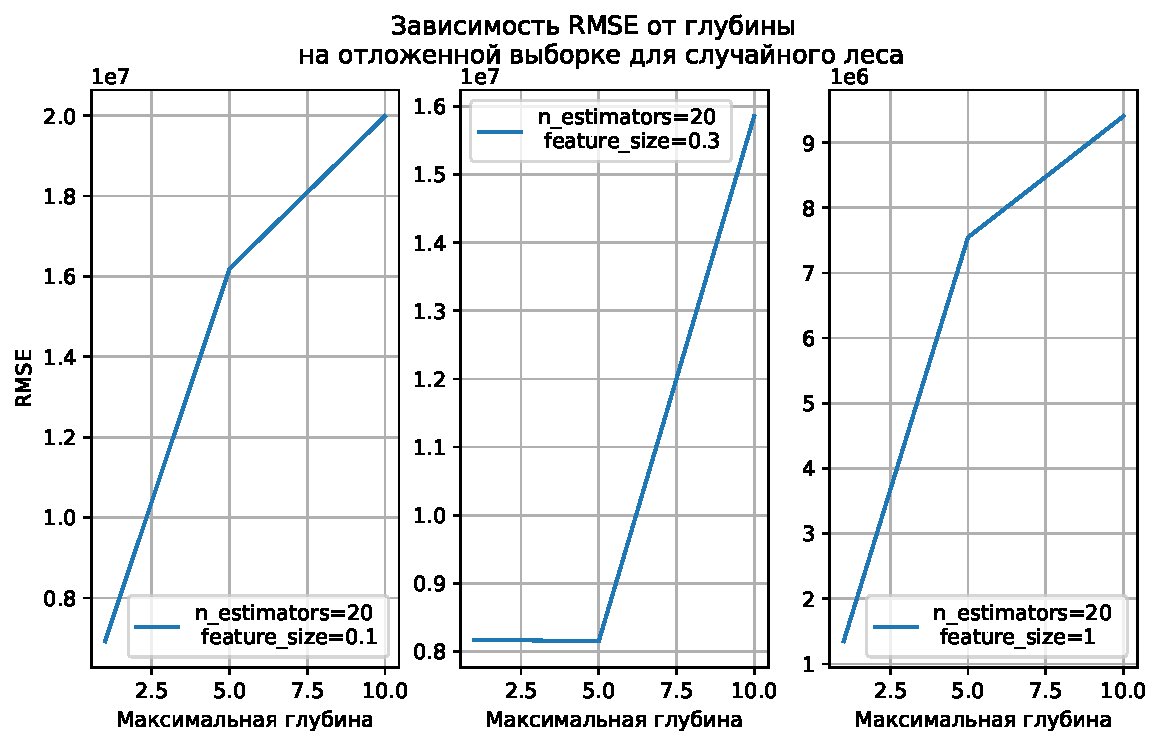
\includegraphics[width=0.8\linewidth]{ex1_3.pdf}
        	\label{fig:mpr}
        	\vspace{-25pt}
\end{figure}

\section{Исследование поведения алгоритма градиентный бустинг.}  


Исследуем зависимость значения функции потерь на отложенной выборке и  времени работы алгоритма в зависимости от следующих параметров:
\begin{itemize}
        \item количество деревьев в ансамбле 
        \item размерность подвыборки признаков для одного дерева
        \item максимальная глубина дерева
        \item выбранный learning\_rate
\end{itemize}


Рассмотрим следующие параметры :
\begin{table}[H]
\begin{tabular}{lllll}
размерность подвыборки признаков: & 0.1 & 0.5 & 1 & 0.3  \\
глубина дерева:  & 1 & 5 & 10 & None  \\
learning\_rate: & 0.1 & 0.5 & 1   \\
\end{tabular}
\end{table}

Количество деревьев рассмотри от 1 до 100


Как видно из рисунка значение RMSE сильно колеблется в зависимость от числа деревьев. С ростом глубины точность также становится хуже. При максимальной глубине 1 и размере подвыборки признаков 10-30\% значение RMSE близки к нулю, но при большей глубине точность лучше при большей размерности подвыборки признаков. Это свзанно с тем, что с ростом глубины модель лучше настраивается, когда признаков больше.
\begin{figure}[H]
        	\centering
        	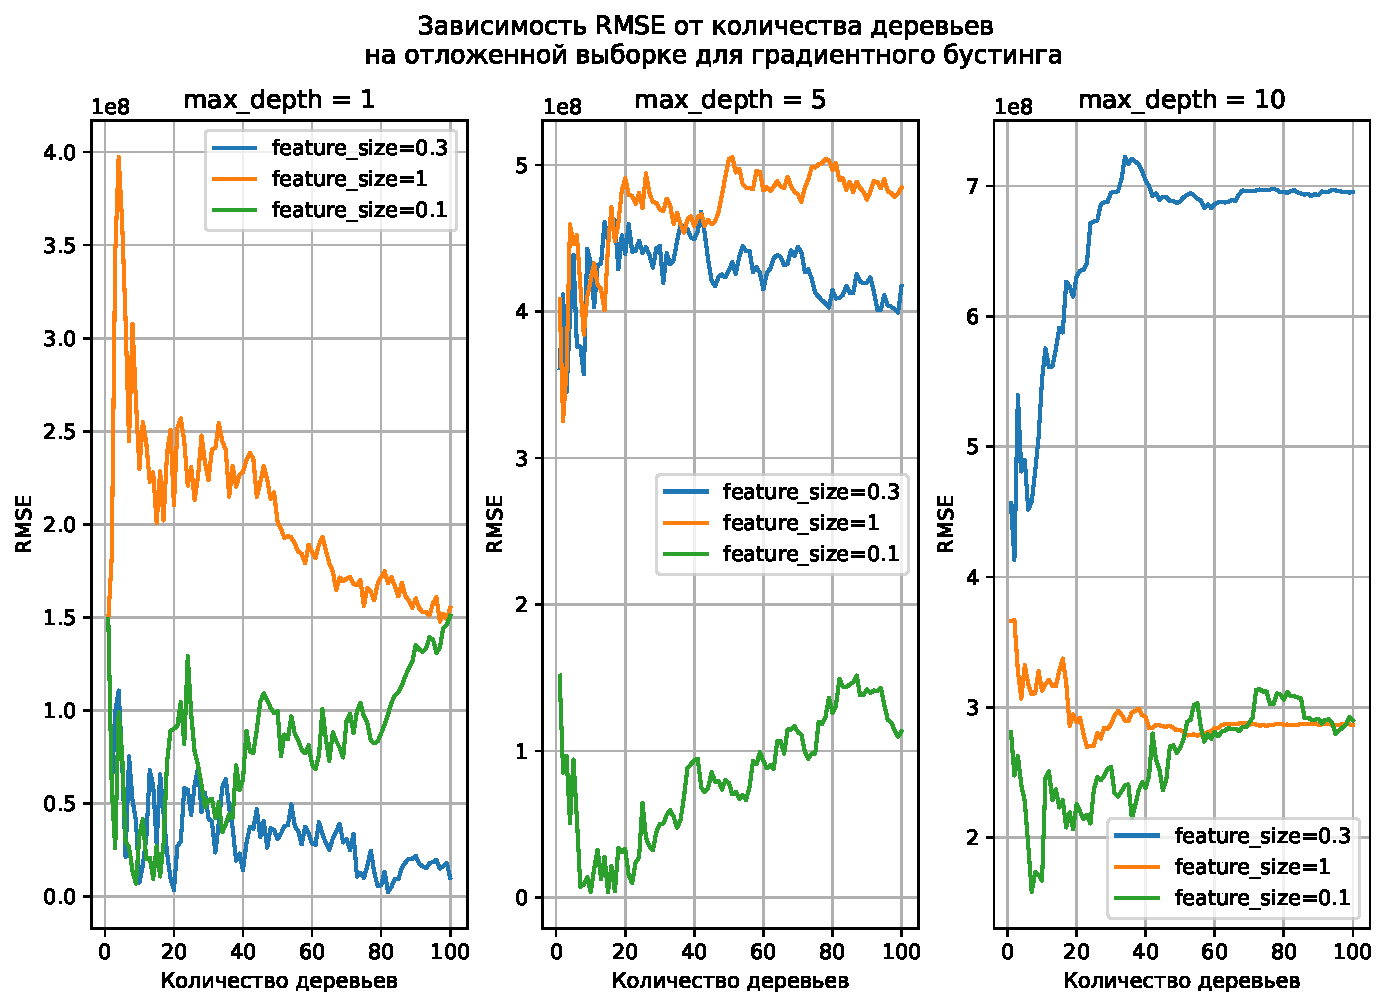
\includegraphics[width=1\linewidth]{ex2_1.pdf}
        	\label{fig:mpr}
        	\vspace{-23pt}
\end{figure}



При неограниченной глубине RMSE больше и колеблется около одного значения. При этом на всем подмножестве признаков становится постоянным, так как алгоритмы получаются достаточно похожими.

\begin{figure}[H]
        	\centering
        	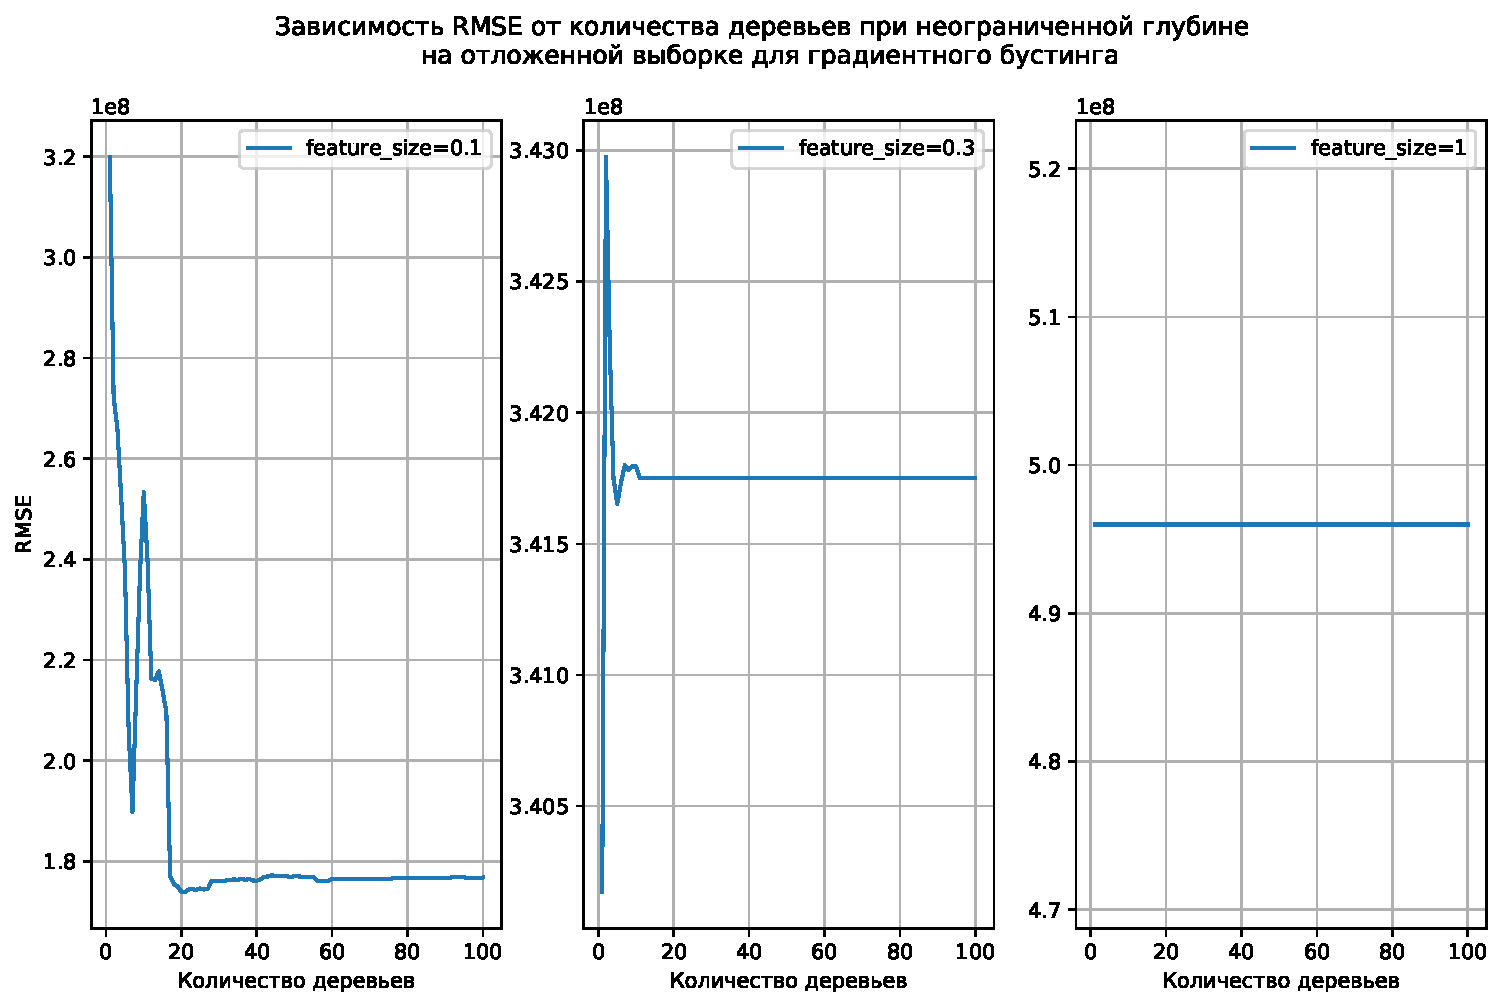
\includegraphics[width=1\linewidth]{ex2_2.pdf}
        	\label{fig:mpr}
        	\vspace{-25pt}
\end{figure}

С ростом глубины и количества деревьев время работы также растет. При этом при неограниченной глубине алгорит работает быстрее, чем при глубине 5 или 10.

\begin{figure}[H]
        	\centering
        	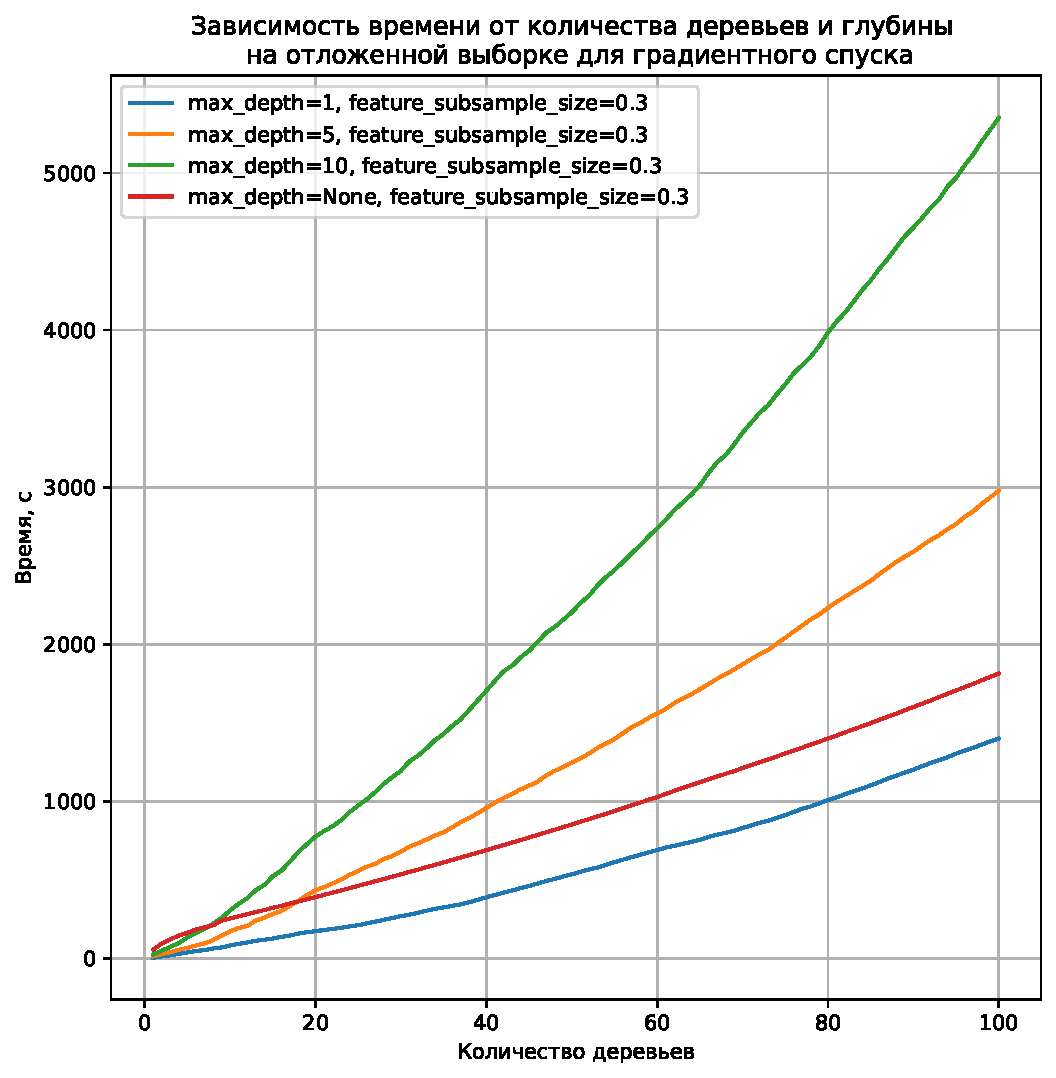
\includegraphics[width=0.7\linewidth]{ex2_3.pdf}
        	\label{fig:mpr}
        	\vspace{-25pt}
\end{figure}

На рисунке ниже показана зависимость значения RMSE от шага обучения learning\_rate. Как видно из графика наилучшая точность достигается при learning\_rate = 0.4. При больших значенияпараметра точность становится хуже. 


\begin{figure}[H]
        	\centering
        	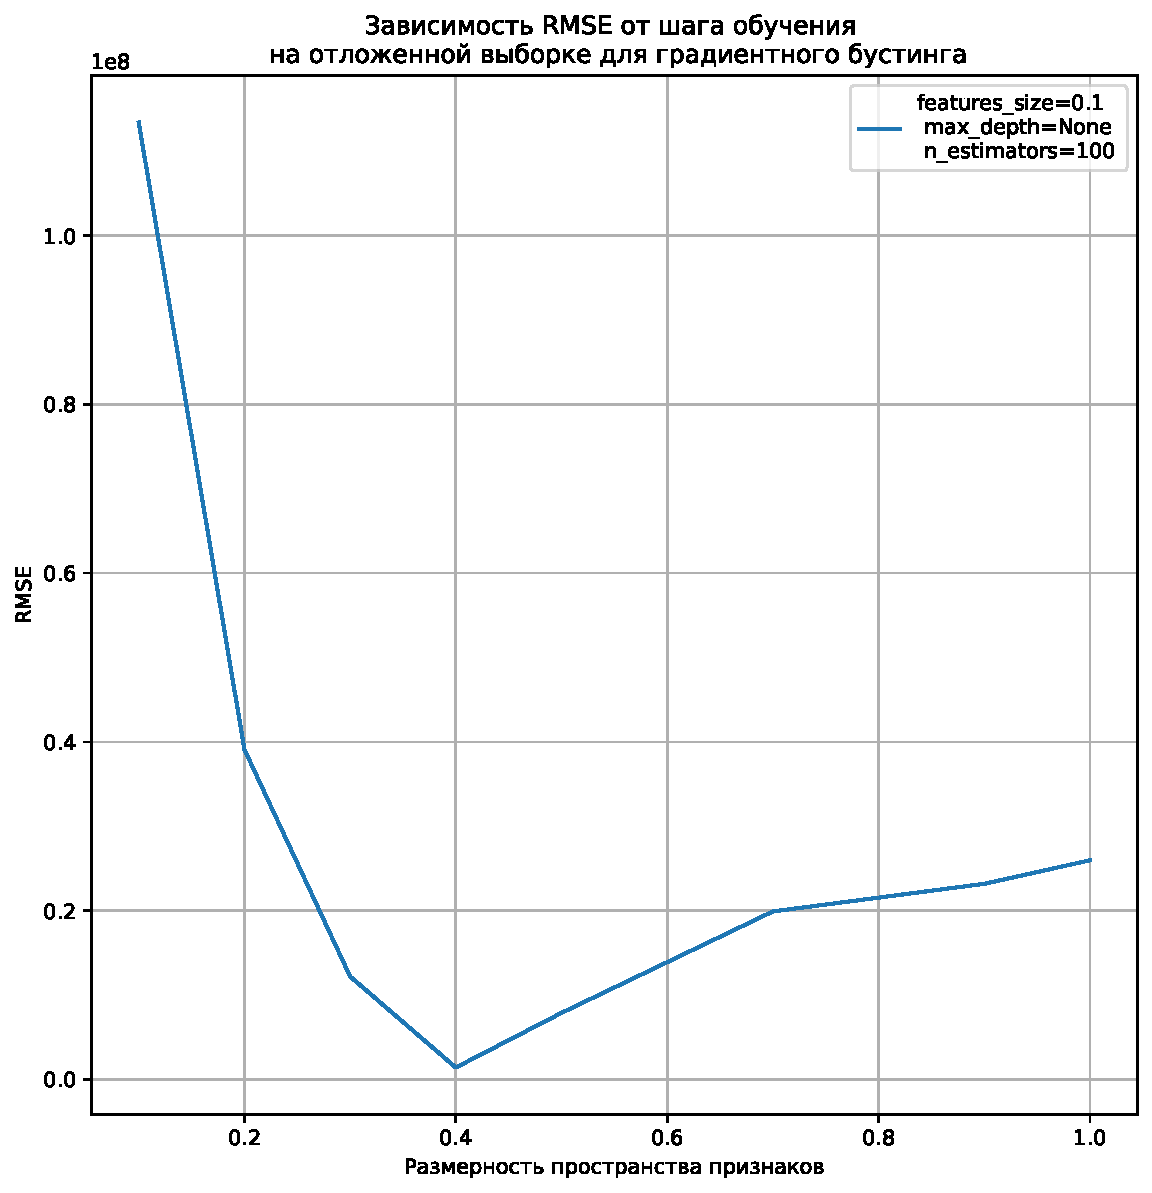
\includegraphics[width=0.78\linewidth]{ex2_6.pdf}
        	\label{fig:mpr}
        	\vspace{-25pt}
\end{figure}

Наилучшее время работы также при значении learning\_rate = 0.4.

\begin{figure}[H]
        	\centering
        	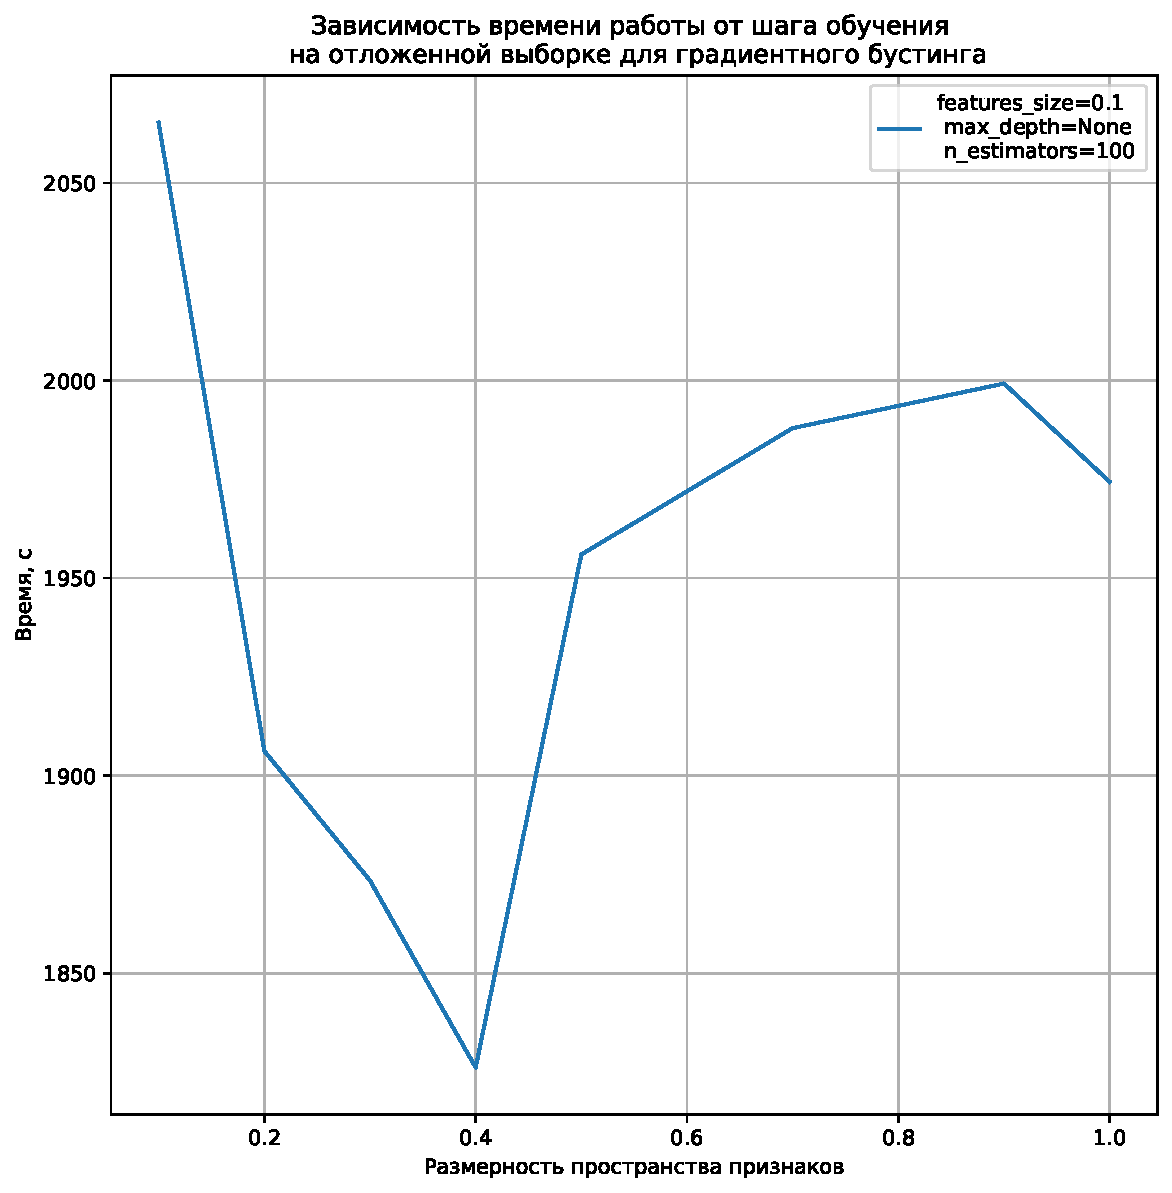
\includegraphics[width=0.7\linewidth]{ex2_7.pdf}
        	\label{fig:mpr}
        	\vspace{-25pt}
\end{figure}



\chapter{Вывод}
    Алгоритмы случайного леса и градиентного бустинга существенно зависят от своих параметров. На наших данных наилучшее значение RMSE достигается при небольшой глубине деревьев. С ростом количества деревьев точность также как правило становится лучше, но при этом возрастает и время работы. Оптимальное значение параметра нужно подбирать в зависимости от ваших целей. 
    Размерность пространства признаков также влияет на качество модели. В алгоритме случайный лес наилучшее точность достигается при большой размерности, в то время как в градиентном бустинге при малой. При неправильно подобранном параметре модель может переобучится.  
\end{document}